% Please add the following required packages to your document preamble:
% \usepackage[table,xcdraw]{xcolor}
% If you use beamer only pass "xcolor=table" option, i.e. \documentclass[xcolor=table]{beamer}
\begin{longtable}[H]{|p{2cm}|p{1.5cm}|p{2cm}|p{2.8cm}|p{6.3cm}|}

\hline
\rowcolor[HTML]{656565} 
\multicolumn{5}{|c|}{\cellcolor[HTML]{656565}{\color[HTML]{FFFFFF} \textbf{Crafting materials}}}                                                                                                                                                                                                    \\ \hline
\rowcolor[HTML]{C0C0C0} 
{\color[HTML]{000000} \textbf{Material}}          & {\color[HTML]{000000} \textbf{Image}} & {\color[HTML]{000000} \textbf{Location}}  & {\color[HTML]{000000} \textbf{Cost}} & {\color[HTML]{000000} \textbf{Brief description}}                                                                    \\ \hline
{\color[HTML]{000000} \textbf{Pink fabric}}       & \raisebox{-0.8\height}{
\includegraphics[height=1.5cm]{Images/CraftingMaterials/pinkFabric}} & {\color[HTML]{000000} Dynamia, Kingsbury} & {\color[HTML]{000000} 5}             & {\color[HTML]{000000} Cheap pink piece of fabric, pretty common and easy to find in every market in the continent}   \\ \hline
{\color[HTML]{000000} \textbf{Yellow fabric}}     & \raisebox{-0.8\height}{
\includegraphics[height=1.5cm]{Images/CraftingMaterials/yellowFabric}} & {\color[HTML]{000000} Dynamia, Kingsbury} & {\color[HTML]{000000} 5}             & {\color[HTML]{000000} Cheap yellow piece of fabric, pretty common and easy to find in every market in the continent} \\ \hline
{\color[HTML]{000000} \textbf{Light blue fabric}} & \raisebox{-0.8\height}{
\includegraphics[height=1.5cm]{Images/CraftingMaterials/lightBlueFabric}} & {\color[HTML]{000000} Dynamia}            & {\color[HTML]{000000} 5}             & {\color[HTML]{000000} Cheap colored piece of fabric, this particular color can be find only in Dynamia}              \\ \hline
{\color[HTML]{000000} \textbf{Grey fabric}}       & \raisebox{-0.8\height}{
\includegraphics[height=1.5cm]{Images/CraftingMaterials/greyFabric}} & Dynamia, Kingsbury                        & 5                                    & {\color[HTML]{000000} Cheap grey piece of fabric, pretty common and easy to find in every market in the continent}   \\ \hline
{\color[HTML]{000000} \textbf{Red fabric}}        & \raisebox{-0.8\height}{
\includegraphics[height=1.5cm]{Images/CraftingMaterials/redFabric}} & Dynamia, Kingsbury                        & 5                                    & {\color[HTML]{000000} Cheap red piece of fabric, pretty common and easy to find in every market in the continent}    \\ \hline
{\color[HTML]{000000} \textbf{Pink wool}}         & \raisebox{-0.8\height}{
\includegraphics[height=1.5cm]{Images/CraftingMaterials/pinkWool}} & Dynamia, Kingsbury                        & 10                                   & {\color[HTML]{000000} Ball of pink yarn, pretty common and easy to find in every market in the continent}            \\ \hline
{\color[HTML]{000000} \textbf{Grey wool}}         & \raisebox{-0.8\height}{
\includegraphics[height=1.5cm]{Images/CraftingMaterials/greyWool}} & Dynamia, Kingsbury                        & 10                                   & {\color[HTML]{000000} Ball of grey yarn, pretty common and easy to find in every market in the continent}            \\ \hline
{\color[HTML]{000000} \textbf{Yellow wool}}       & \raisebox{-0.8\height}{
\includegraphics[height=1.5cm]{Images/CraftingMaterials/yellowWool}} & Dynamia, Kingsbury                        & 10                                   & {\color[HTML]{000000} Ball of yellow yarn, pretty common and easy to find in every market in the continent}          \\ \hline
{\color[HTML]{000000} \textbf{Black wool}}        & \raisebox{-0.8\height}{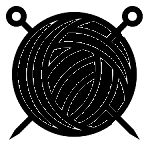
\includegraphics[height=1.5cm]{Images/CraftingMaterials/blackWool}} & Kingsbury                                 & 10                                   & {\color[HTML]{000000} Ball of red yarn, this particular color can be find only in Kingsbury}                         \\ \hline
{\color[HTML]{000000} \textbf{Red wool}}          & \raisebox{-0.8\height}{
\includegraphics[height=1.5cm]{Images/CraftingMaterials/redWool}} & Dynamia, Kingsbury                        & 10                                   & {\color[HTML]{000000} Ball of red yarn, pretty common and easy to find in every market in the continent}             \\ \hline
{\color[HTML]{000000} \textbf{White wool}}          & \raisebox{-0.8\height}{
\includegraphics[height=1.5cm]{Images/CraftingMaterials/whiteWool}} & Dynamia, Kingsbury                        & 10                                   & {\color[HTML]{000000} Ball of white yarn, pretty common and easy to find in every market in the continent}             \\ \hline
{\color[HTML]{000000} \textbf{Leather}}           & \raisebox{-0.8\height}{
\includegraphics[height=1.5cm]{Images/CraftingMaterials/leather}} & Dynamia, Kingsbury (only in few stands)   & 15                                   & {\color[HTML]{000000}                                                                                             Tanned leather used for belts and particular hats, a bit expensive and not so easy to find }\\ \hline
{\color[HTML]{000000} \textbf{Wolf fur}}          & \raisebox{-0.8\height}{
\includegraphics[height=1.5cm]{Images/CraftingMaterials/wolfFur}} & Kingsbury (only in few stands)            & 35                                   & {\color[HTML]{000000}                                                                                    Fur of grey wolf used for soft and warm dresses and hats, rare to find and definitely expensive} \\ \hline
{\color[HTML]{000000} \textbf{Bear fur}}          & \raisebox{-0.8\height}{
\includegraphics[height=1.5cm]{Images/CraftingMaterials/bearFur}} & Dynamia (only in few stands)              & 35                                   & {\color[HTML]{000000}                                                                                            Fur of brown grizzly used for soft and warm dresses and hats, rare to find and definitely expensive } \\ \hline

\end{longtable}